\documentclass[letter,11pt]{article}
\usepackage{xcolor}
\usepackage{float}
\usepackage{amsthm}
\usepackage{amssymb}
\usepackage{wrapfig}
\usepackage{tabularx}
\usepackage{titlesec}
\usepackage[symbol]{footmisc}
\usepackage{tikz}
\usepackage{pgfplots}
\usepackage{pgfplotstable}
\usepackage{geometry}
\usepackage{verbatim}
\usepackage{enumitem}
\usepackage{fancyhdr}
\usepackage{multicol}
\usepackage{systeme}
\usepackage{booktabs}
\usepackage{graphicx}
\usepackage{mathtools}
\usepackage{booktabs}
\usepackage{svg}
\usepackage[most]{tcolorbox}
\usepackage[T1]{fontenc}
\usetikzlibrary{trees}
\setlength{\multicolsep}{0pt} 
\pagestyle{fancy}
%\fancyhf{} % clear all header and footer fields
\fancyhead{}\fancyfoot{}
\fancyhead[R]{\textbf{\thepage}}
\fancyhead[L]{Aiden M. Rosenberg, MMXXIV A.D. }
\addtolength{\headwidth}{3cm}
\addtolength{\headheight}{1cm}

\renewcommand{\headrulewidth}{1pt}
\renewcommand{\footrulewidth}{0pt}
\geometry{left=1.5cm, top=2.5cm, right=1.5cm, bottom=1.25cm}
\usepackage{amsthm}
\usepackage[most]{tcolorbox}

\pgfplotsset{compat=1.18}

\usepackage{tasks}
\settasks{
	label=(\Alph*.),
	label-width=21pt
}

\raggedright
\setlength{\tabcolsep}{0in}

% Sections formatting
\titleformat{\section}{
  \vspace{-4pt}\scshape\raggedright\large
}{}{0em}{}[\color{black}\titlerule \vspace{-7pt}]

\titleformat{\subsection}[block]
  { \vspace{4pt}\bfseries\centering}
  {}{0em}{}

\newcommand{\pvec}[1]{\vec{#1}\mkern2mu\vphantom{#1}}

\makeatletter
\renewcommand*\env@matrix[1][\arraystretch]{%
  \edef\arraystretch{#1}%
  \hskip -\arraycolsep
  \let\@ifnextchar\new@ifnextchar
  \array{*\c@MaxMatrixCols c}}
\makeatother

\theoremstyle{definition}
\newtheorem{definition}{Definition}[section]

\newtheorem{theorem}{Theorem}[section]

\DeclareTotalTColorBox{\mysidebox}{ O{} +m +m }{
bicolor,colback=white,colbacklower=yellow!10,
fonttitle=\bfseries,center title,
sidebyside,
code={\sbox{\mysavebox}{#2}},
lefthand width=\wd\mysavebox,
drop lifted shadow,
#1
}
{\usebox{\mysavebox}\tcblower#3}


\begin{document}

\thispagestyle{empty}

%----------HEADING-----------------

\parbox{2.35cm}{%
	\includesvg[width=2.3cm]{logo.svg}
}
\parbox{0.3cm}{\hspace{0.3cm}}
\parbox{\dimexpr\linewidth-5cm\relax}{
	\setlength{\tabcolsep}{0.5em}
	\def\arraystretch{1.25}
	\begin{tabular}{@{}llll@{}}
		\toprule
		\multicolumn{4}{c}
		{\hspace{-0.5em}\textbf{Assignment}: Worksheet 7 (\S6.2 - \S6.5)} \\ \midrule
		\textbf{Name:}   & Aiden M. Rosenberg  & \textbf{Professor:} & Dr. Terry Bridgman Ph.D \\
		\textbf{Course:} & Linear Algebra          & \textbf{Date:}      & \today \: A.D.   \\ \bottomrule
	\end{tabular}}
\parbox{0.3cm}{\hspace{0.3cm}}
\vspace{1cm}

\section{Problem 1}
What is the orthogonal projection of $\vec{\boldsymbol{y}}=\begin{bmatrix}-24\\ -10\end{bmatrix}$ onto $\vec{\boldsymbol{u}}=\begin{bmatrix}3 \\ -15\end{bmatrix}$?

$$\boxed{\hat{\boldsymbol{y}} = \operatorname{proj}_{\vec{\boldsymbol{u}}} \left(\vec{\boldsymbol{v}}\right) = \frac{\left\langle\vec{\boldsymbol{y}},\vec{\boldsymbol{u}}_{1}\right\rangle}{\left\langle\vec{\boldsymbol{u}}_{1}, \vec{\boldsymbol{u}}_{1}\right\rangle}\vec{\boldsymbol{u}}_{1} = \frac{1}{3} \begin{bmatrix} 3 \\-15 \end{bmatrix} = \begin{bmatrix} 1 \\-5 \end{bmatrix}}$$

\section{Problem 2}
Let $W=\operatorname{Span}\left\{\vec{\boldsymbol{u}}_{1}, \vec{\boldsymbol{u}}_{2}\right\}$ where $\vec{\boldsymbol{u}}_{1}=\begin{bmatrix} 2 \\ 2 \\ -1 \end{bmatrix}$ and $\vec{\boldsymbol{u}}_{2}=\begin{bmatrix} -1 \\ 3 \\ 4 \end{bmatrix}$, and let $\vec{\boldsymbol{y}}=\begin{bmatrix} 11 \\ 9 \\ 22 \end{bmatrix}$.

Write $\vec{\boldsymbol{y}}$ as a sum of a vector in $W$ and a vector in $W^{\perp}$.

\begin{tcolorbox}[boxrule=1mm,enhanced jigsaw, breakable,before=\hfill,after=\hfill,adjusted title={Problem 2 solution}]
    \begin{definition}[The Orthogonal Decomposition Theorem]
        Let $W$ be a subspace of $\mathbb{R}^n$. Then each $\vec{\boldsymbol{y}}$ in $\mathbb{R}^n$ can be written uniquely in the form  $\vec{\boldsymbol{y}}=\hat{\boldsymbol{y}}+\vec{\boldsymbol{z}}$ where $\hat{\boldsymbol{y}}$ is in $W$ and $\vec{\boldsymbol{z}}$ is in $W^{\perp}$. In fact, if $\left\{\vec{\boldsymbol{u}}_1, \ldots, \vec{\boldsymbol{u}}_p\right\}$ is any orthogonal basis of $W$, then
        
    $$\hat{\boldsymbol{y}}=\frac{\vec{\boldsymbol{y}} \cdot \vec{\boldsymbol{u}}_1}{\vec{\boldsymbol{u}}_1 \cdot \boldsymbol{u}_1} \vec{\boldsymbol{u}}_1+\cdots+\frac{\vec{\boldsymbol{y}} \cdot \vec{\boldsymbol{u}}_p}{\vec{\boldsymbol{u}}_p \cdot \vec{\boldsymbol{u}}_p} \vec{\boldsymbol{u}}_p$$

    and $\vec{\boldsymbol{z}}=\vec{\boldsymbol{y}}-\hat{\boldsymbol{y}}$.
    \end{definition}
    \tcblower
    The orthogonal projection of $\vec{\boldsymbol{y}}$ onto $W$ is

    \begin{align*}
        \hat{y} &= \frac{\vec{\boldsymbol{y}} \cdot \vec{\boldsymbol{u}}_1}{\vec{\boldsymbol{u}}_1 \cdot \boldsymbol{u}_1} \vec{\boldsymbol{u}}_1+\cdots+\frac{\vec{\boldsymbol{y}} \cdot \vec{\boldsymbol{u}}_2}{\vec{\boldsymbol{u}}_2 \cdot \vec{\boldsymbol{u}}_2} \vec{\boldsymbol{u}}_2\\
        &= 2\begin{bmatrix} 2\\2\\-1\end{bmatrix} + 4\begin{bmatrix} -1\\3\\-4\end{bmatrix} =\begin{bmatrix} 4\\4\\-2\end{bmatrix}+\begin{bmatrix} -4\\12\\16\end{bmatrix} = \begin{bmatrix} 0\\16\\14\end{bmatrix}
    \end{align*}
    Also,
     $$\vec{\boldsymbol{y}} - \hat{\boldsymbol{y}} = \begin{bmatrix} 11\\9\\22\end{bmatrix} - \begin{bmatrix} 0\\16\\14\end{bmatrix} = \begin{bmatrix} 11\\-7\\8\end{bmatrix}$$
     
     Definition 2.1 ensures that $\vec{\boldsymbol{y}} - \hat{\boldsymbol{y}}$ is in $W^{\perp}$. The desired decomposition of $\vec{\boldsymbol{y}}$ is

     $$\boxed{\vec{\boldsymbol{y}} = \begin{bmatrix} 11\\9\\22\end{bmatrix} = \begin{bmatrix} 0\\16\\14\end{bmatrix}+\begin{bmatrix} 11\\-7\\8\end{bmatrix}}$$ \qed
\end{tcolorbox}

\section{Problem 3}
 For each of the following statements, indicate if the statement is \textbf{True} or \textbf{False}\footnote{ If a statement is not always true, then it can be considered a false statement.}.
\begin{enumerate}[label = \roman*.]
    \item If $V$ is a vector space of dimension $d$, then every basis for $V$ must have the same number of vectors.
    \item If $V$ is a vector space of dimension $d$, and $\left\{\vec{\boldsymbol{v}}_{1}, \ldots, \vec{\boldsymbol{v}}_{d}\right\}$ are $d$ linearly independent vectors in $V$ , then they must span $V$.
    \item The dimension of $\mathbb{P}_{4}$ is 4 .
\end{enumerate}

\begin{tcolorbox}[boxrule=1mm,enhanced jigsaw, breakable,before=\hfill,after=\hfill,adjusted title={Problem 3 solutions}]
    \begin{definition}
        If $V$ is spanned by a finite set, then $V$ is said to be \underline{finite-dimensional}, and the \underline{dimension} of $V$, written as $\operatorname{dim} V$ , is the number of vectors in a basis for $V$. The dimension of the zero vector space $\left\{\boldsymbol{0}\right\}$ is defined to be zero. If $V$ is not spanned by a finite set, then $V$ is said to be \underline{infinite-dimensional}.
    \end{definition}
    \begin{theorem}
         If a vector space $V$ has a basis $\mathcal{B} = \left\{\vec{\boldsymbol{b}}_1, \ldots, \vec{\boldsymbol{b}}_n\right\}$, then any set in $V$ containing more than $n$ vectors must be linearly dependent.
    \end{theorem}
    \begin{theorem}
        If a vector space $V$ has a basis of $n$ vectors, then every basis of V must consist of exactly $n$ vectors. If a vector space $V$ has a basis of $n$ vectors, then every basis of $V$ must consist of exactly $n$ vectors.
    \end{theorem}
    \tcblower
    \begin{enumerate}
        \item \textbf{True}, by definition 3.1.
        \item \textbf{True}, since both theorems 3.1 and 3.2 are satisfied. 
        \item \textbf{False}, rather the $\operatorname{dim}\mathbb{P}_{n} = n+1$, thus the dimension would be $4$.
    \end{enumerate}
\end{tcolorbox}
\newpage
\section{Problem 4}
Consider the following set of polynomials in $\mathbb{P}_{2}$,

$$S=\left\{1+t^{2}, t+t^{2}, 1+2 t+t^{2}\right\}$$

Is $S$ a basis for $\mathbb{P}_{2}$? Why or why not?

\begin{tcolorbox}[boxrule=1mm,enhanced jigsaw, breakable,before=\hfill,after=\hfill,adjusted title={Problem 4 solutions}]
A typical element $\vec{\boldsymbol{p}}$ of $\mathbb{P}_2$ has the form $\vec{\boldsymbol{p}}(t) = a_{0}+a_{1}t+a_{2}t^2$. Since $\vec{\boldsymbol{p}}$ is displayed previously as a linear combination of the standard basis vectors, we conclude that

$$\left[\vec{\boldsymbol{p}}\right]_{\mathcal{B}} = \begin{bmatrix} a_0 \\ a_{1} \\ a_{2}\end{bmatrix}$$.
\tcblower
The coordinate mapping from above produces the coordinate vectors, $(1,0,1)$, $(0,1,1)$, and $(1,2,1)$ respectively. Writing these vectors as the \textit{columns} of matrix $A$, we can determine their independence by row reducing the augmented matrix for $A\vec{\boldsymbol{x}} = \vec{\boldsymbol{0}}$:
$$\begin{bmatrix}
    1 & 0 & 1 & 0\\
    0 & 1 & 2 & 0\\
    1 & 1 & 1 & 0
\end{bmatrix} \leadsto
\begin{bmatrix}
    1 & 0 & 0 & 0\\
    0 & 1 & 0 & 0\\
    0 & 0 & 1 & 0
\end{bmatrix}
$$
The columns of $A$ are linearly independent, so the corresponding polynomials are linearly independent, therefore $S$ is a basis for $\mathbb{P}_{2}$.
\end{tcolorbox}
\newpage
\section{Problem 5}
Let $\boldsymbol{x}_{1}=\begin{bmatrix}1 \\ -1 \\ -1 \\ 1 \\ 1\end{bmatrix}, \boldsymbol{x}_{2}=\begin{bmatrix}2 \\ 1 \\ 4 \\ -4 \\ 2\end{bmatrix}$, and $\boldsymbol{x}_{3}=\begin{bmatrix}5 \\ -4 \\ -3 \\ 7 \\ 1\end{bmatrix}$, and let $W=\operatorname{Span}\left\{\boldsymbol{x}_{1}, \boldsymbol{x}_{2}, \boldsymbol{x}_{3}\right\}$.

Find an orthogonal basis $\mathcal{B}$ for $W$.

\begin{tcolorbox}[boxrule=1mm,enhanced jigsaw, breakable,before=\hfill,after=\hfill,adjusted title={Problem 5 solutions}]
  \begin{definition}[The Gram-Schmidt Process]
      Given a basis $\left\{\vec{\boldsymbol{x}}_1, \ldots, \vec{\boldsymbol{x}}_p\right\}$ for a nonzero subspace $W$ of $\mathbb{R}^n$, define
\begin{align*}
\vec{\boldsymbol{v}}_1 & =\vec{\boldsymbol{x}}_1 \\
\vec{\boldsymbol{v}}_2 & =\vec{\boldsymbol{x}}_2-\frac{\vec{\boldsymbol{x}}_2 \cdot \vec{\boldsymbol{v}}_1}{\vec{\boldsymbol{v}}_1 \cdot \vec{\boldsymbol{v}}_1} \vec{\boldsymbol{v}}_1 \\
\vec{\boldsymbol{v}}_3 & =\vec{\boldsymbol{x}}_3-\frac{\vec{\boldsymbol{x}}_3 \cdot \vec{\boldsymbol{v}}_1}{\vec{\boldsymbol{v}}_1 \cdot \vec{\boldsymbol{v}}_1} \vec{\boldsymbol{v}}_1-\frac{\vec{\boldsymbol{x}}_3 \cdot \vec{\boldsymbol{v}}_2}{\vec{\boldsymbol{v}}_2 \cdot \vec{\boldsymbol{v}}_2} \vec{\boldsymbol{v}}_2 \\
& \vdots \\
\vec{\boldsymbol{v}}_p & =\vec{\boldsymbol{x}}_p-\frac{\vec{\boldsymbol{x}}_p \cdot \vec{\boldsymbol{v}}_1}{\vec{\boldsymbol{v}}_1 \cdot \vec{\boldsymbol{v}}_1} \vec{\boldsymbol{v}}_1-\frac{\vec{\boldsymbol{x}}_p \cdot \vec{\boldsymbol{v}}_2}{\vec{\boldsymbol{v}}_2 \cdot \vec{\boldsymbol{v}}_2} \vec{\boldsymbol{v}}_2-\cdots-\frac{\vec{\boldsymbol{x}}_p \cdot \vec{\boldsymbol{v}}_{p-1}}{\vec{\boldsymbol{v}}_{p-1} \cdot \vec{\boldsymbol{v}}_{p-1}} \vec{\boldsymbol{v}}_{p-1}
\end{align*}

Then $\left\{\vec{\boldsymbol{v}}_1, \ldots, \vec{\boldsymbol{v}}_p\right\}$ is an orthogonal basis for $W$.
\end{definition}
\tcblower
Applying the Gram-Schmidt Process for the problem above:
\begin{align*}
\vec{\boldsymbol{v}}_1 & = \vec{\boldsymbol{x}}_1 = \begin{bmatrix}1\\-1\\-1\\1\\1 \end{bmatrix}\\
\vec{\boldsymbol{v}}_2 & =\vec{\boldsymbol{x}}_2-\frac{\vec{\boldsymbol{x}}_2 \cdot \vec{\boldsymbol{v}}_1}{\vec{\boldsymbol{v}}_1 \cdot \vec{\boldsymbol{v}}_1} \vec{\boldsymbol{v}}_1 = \begin{bmatrix}2\\1\\4\\-4\\2 \end{bmatrix} + \begin{bmatrix}1\\-1\\-1\\1\\1 \end{bmatrix} = \begin{bmatrix}3\\0\\3\\-3\\3 \end{bmatrix}\\
\vec{\boldsymbol{v}}_3 & =\vec{\boldsymbol{x}}_3-\frac{\vec{\boldsymbol{x}}_3 \cdot \vec{\boldsymbol{v}}_1}{\vec{\boldsymbol{v}}_1 \cdot \vec{\boldsymbol{v}}_1} \vec{\boldsymbol{v}}_1-\frac{\vec{\boldsymbol{x}}_3 \cdot \vec{\boldsymbol{v}}_2}{\vec{\boldsymbol{v}}_2 \cdot \vec{\boldsymbol{v}}_2} \vec{\boldsymbol{v}}_2 = \begin{bmatrix}5\\-4\\-3\\7\\1 \end{bmatrix} - 4\begin{bmatrix}1\\-1\\-1\\1\\1 \end{bmatrix} + \frac{1}{3}\begin{bmatrix}3\\0\\3\\-3\\3 \end{bmatrix} = \begin{bmatrix}2\\0\\2\\2\\-2 \end{bmatrix}
\end{align*}
Thus, an orthogonal basis $\mathcal{B}$ for $W$ is
$$\boxed{\mathcal{B} = \left\{\begin{bmatrix}1\\-1\\-1\\1\\1 \end{bmatrix},\begin{bmatrix}3\\0\\3\\-3\\3 \end{bmatrix} \begin{bmatrix}2\\0\\2\\2\\-2 \end{bmatrix}\right\}}$$
\end{tcolorbox}

\section{Problem 6}
Consider the following set of data points.

$$(1,0),(2,1),(4,2), (5,3)$$
\begin{enumerate}
    \item Find the equation $y=\beta_{0}+\beta_{1}x$ of the least squares line that best fits these given data points. Use the Normal Equations. Clearly show how you set up the system of equations. You do not need to show row operations. Your final answer should be the equation of the line.
    \item Plot the data and the line of best fit on the same axes.
    \item What is the least-squares error of this line?
\end{enumerate}

\begin{tcolorbox}[boxrule=1mm,enhanced jigsaw, breakable,before=\hfill,after=\hfill,adjusted title={Problem 6 solutions}]
    If the data points were on the line, the parameters $\beta_{0}$ and $\beta_{1}$ would satisfy the equations

\begin{center}
\begin{tabular}{ccc}
\toprule
Predicted $y$-value & \hspace{1cm} & Observed $y$-value \\ \midrule
$\beta_{0}+\beta_{1}x_{1}$ & $=$ & $y_{1}$  \\
$\beta_{0}+\beta_{1}x_{2}$ & $=$ & $y_{2}$  \\
$\vdots$                   &     & $\vdots$ \\
$\beta_{0}+\beta_{1}x_{n}$ & $=$ & $y_{n}$  \\ \bottomrule
\end{tabular}
\end{center}
We can write this system as
\begin{equation}
    X \boldsymbol{\beta}=\boldsymbol{y}, \quad\text{where} \quad X=\begin{bmatrix} 1 & x_1 \\ 1 & x_2 \\ \vdots & \vdots \\ 1 & x_n\end{bmatrix}, \quad \boldsymbol{\beta}=\begin{bmatrix}\beta_0 \\ \beta_1\end{bmatrix}, \quad \vec{\boldsymbol{y}}=\begin{bmatrix}y_1 \\ y_2 \\ \vdots \\ y_n\end{bmatrix}
\end{equation}

\tcblower
Use the $x$-coordinates of the data to build the design matrix $X$ in (1) and
the y-coordinates to build the observation vector $y$:

\begin{equation*}
    X=\begin{bmatrix} 1 & 1\\ 1 & 2\\ 1 & 4\\ 1 & 5 \end{bmatrix}, \quad \vec{\boldsymbol{y}} =\begin{bmatrix} 0\\ 1\\2\\3 \end{bmatrix}
\end{equation*}
For the least-squares solution of $X\boldsymbol{\beta} = \vec{\boldsymbol{y}}$, obtain the normal equations (with the new
notation):
$$X^{T}X\boldsymbol{\beta} = X^{T}\vec{\boldsymbol{y}}$$
That is, compute 

$$X^{T}X = 
    \begin{bmatrix}
        1 & 1 & 1 & 1\\
        1 & 2 & 4 & 5
    \end{bmatrix}
    \begin{bmatrix} 
        1 & 1\\
        1 & 2\\
        1 & 4\\
        1 & 5
    \end{bmatrix} = 
    \begin{bmatrix} 
        4 & 12 \\
        12 & 46
    \end{bmatrix}$$

$$X^{T}\vec{\boldsymbol{y}} = 
    \begin{bmatrix}
        1 & 1 & 1 & 1\\
        1 & 2 & 4 & 5
    \end{bmatrix}
    \begin{bmatrix} 
       0\\ 1\\ 2\\ 3
    \end{bmatrix} = 
    \begin{bmatrix} 
        6 \\ 25
    \end{bmatrix}$$
The normal equations are

$$\begin{bmatrix} 
        4 & 12 \\
        12 & 46
    \end{bmatrix}
    \begin{bmatrix} 
        \beta_{0}\\ \beta_{1}
    \end{bmatrix} = 
    \begin{bmatrix} 
        6 \\ 25
    \end{bmatrix}$$
Hence
$$\begin{bmatrix} 
        \beta_{0}\\ \beta_{1}
    \end{bmatrix}
    = \begin{bmatrix}
        4 & 12 \\
        12 & 46
    \end{bmatrix}^{-1}\begin{bmatrix} 
        6 \\ 25
    \end{bmatrix}= \frac{1}{40}\begin{bmatrix}
        46 & -12 \\
        -12 & 4
    \end{bmatrix}\begin{bmatrix} 
        6 \\ 25
    \end{bmatrix}= \frac{1}{40}\begin{bmatrix} 
        -24 \\ 28
    \end{bmatrix} = \begin{bmatrix}[1.5]
        -\frac{3}{5} \\ \frac{7}{10}
    \end{bmatrix}
    $$
Thus the least-squares line has the equation
$$y=-\frac{3}{5}+\frac{7}{10}x$$
\qed

\begin{tcolorbox}[boxrule=0.25mm,enhanced jigsaw, breakable, colframe=red!75!black,colback=white,before=\hfill,after=\hfill]
    \centering
    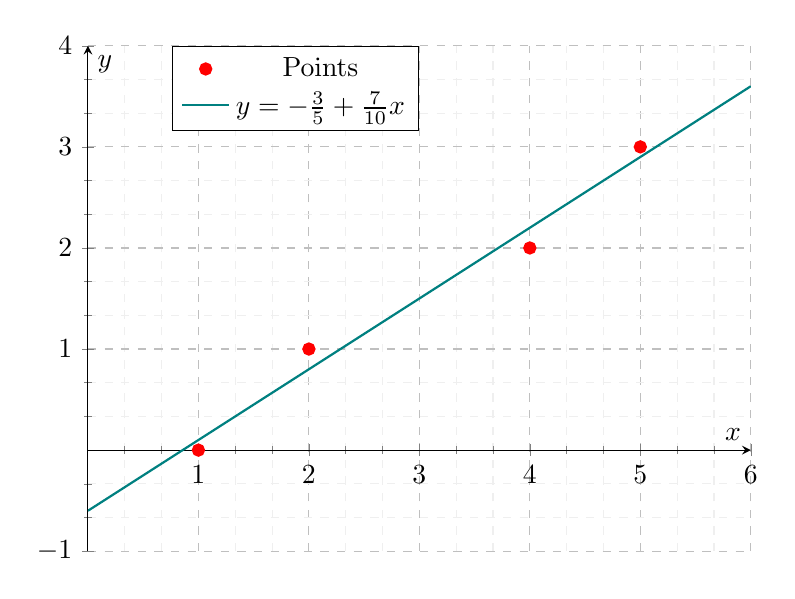
\begin{tikzpicture}
        \begin{axis}[every axis plot/.append style={thick},
            axis lines = middle,
            xlabel = $x$,
            ylabel = $y$,
            xmin=0, xmax=6,
            ymin=-1, ymax=4,
            minor tick num=2,
            width=10cm,
            height=8cm,
            grid style=dashed,
            major grid style = {lightgray},
            minor grid style = {lightgray!25},
            legend style={at={(0.5,1)}}, 
            ymajorgrids=true,
            xmajorgrids=true,
            grid=both
        ]
        
        % Points
        \addplot[red, only marks, mark=*] coordinates {(1,0) (2,1) (4,2) (5,3)};
        
        % Line
        \addplot[domain=0:6, samples=100, color=teal] {-3/5 + (7/10)*x};
        
        \addlegendentry{Points}
        \addlegendentry{$y=-\frac{3}{5} + \frac{7}{10}x$}
        \end{axis}
    \end{tikzpicture}
\end{tcolorbox}

The least-squares error is given by the expression $||\vec{\boldsymbol{y}} - X\boldsymbol{\beta}||$.
$$\vec{\boldsymbol{y}} - X\boldsymbol{\beta} = \begin{bmatrix} 0\\ 1\\ 2\\ 3 \end{bmatrix} - \begin{bmatrix} 1 & 1\\ 1 & 2\\ 1 & 4\\ 1 & 5 \end{bmatrix}\begin{bmatrix}[1.5]
        -\frac{3}{5} \\ \frac{7}{10}
    \end{bmatrix} = \begin{bmatrix}[1.5] 0\\ 1\\ 2\\ 3 \end{bmatrix} - \begin{bmatrix}[1.5] \frac{1}{10}\\ \frac{4}{5}\\ \frac{11}{5}\\ \frac{29}{10} \end{bmatrix} = \begin{bmatrix}[1.5] -\frac{1}{10}\\ \frac{1}{5}\\ -\frac{1}{5}\\ \frac{1}{10} \end{bmatrix}$$

$$||\vec{\boldsymbol{y}} - X\boldsymbol{\beta}|| = \sqrt{\left(-\frac{1}{10}\right)^{2}+\left(\frac{1}{5}\right)^{2}+\left(-\frac{1}{5}\right)^{2}+\left(\frac{1}{10}\right)^{2}} = \frac{\sqrt{10}}{10}$$
\end{tcolorbox}

\newpage
\section{Problem 7}
Find the least squares solution(s) for $A \vec{\boldsymbol{x}}=\vec{\boldsymbol{b}}$ where

$$ A=\begin{bmatrix} 1 & 1 & 0 \\ 1 & 1 & 0 \\ 1 & 0 & 1 \\ 1 & 0 & 1 \end{bmatrix} \text { and } \vec{\boldsymbol{b}}= \begin{bmatrix} 1 \\ 3 \\ 8 \\ 2 \end{bmatrix} $$

\begin{tcolorbox}[boxrule=1mm,enhanced jigsaw, breakable,before=\hfill,after=\hfill,adjusted title={Problem 7 solutions}]
Compute:

$$A^{T}A = \begin{bmatrix} 1 & 1 & 1 & 1\\ 1 & 1 & 0 & 0\\ 0 & 0 & 1 & 1 \end{bmatrix}\begin{bmatrix} 1 & 1 & 0 \\ 1 & 1 & 0 \\ 1 & 0 & 1 \\ 1 & 0 & 1 \end{bmatrix} = \begin{bmatrix} 4 & 2 & 2\\ 2 & 2 & 0\\ 2 & 0 & 2 \end{bmatrix}$$

$$A^{T}\vec{\boldsymbol{b}} = \begin{bmatrix} 1 & 1 & 1 & 1\\ 1 & 1 & 0 & 0\\ 0 & 0 & 1 & 1 \end{bmatrix}\begin{bmatrix} 1 \\ 2 \\ 8 \\2 \end{bmatrix} = \begin{bmatrix} 14 \\ 4 \\ 10 \end{bmatrix}$$

The augmented matrix for $A^{T}A\vec{\boldsymbol{x}}=A^{T} \vec{\boldsymbol{b}}$ is
    $$\begin{bmatrix}
        4 & 2 & 2 & 14\\
        2 & 2 & 0 & 4 \\
        2 & 0 & 2 & 10
    \end{bmatrix} \leadsto 
    \begin{bmatrix}
        1 & 0 & 1 & 5\\
        0 & 1 & -1 & -3 \\
        0 & 0 & 0 & 0
    \end{bmatrix}$$

The general solution is $x_{1} = 5 - x_{3}$, $x_{2} = -3 + x_{3}$, and $x_3$ is free. So the general least-squares solution of $A\vec{\boldsymbol{x}} = \vec{\boldsymbol{b}}$ has the form

$$\hat{\boldsymbol{x}} = \begin{bmatrix}5 \\ -3 \\ 0\end{bmatrix} + \vec{\boldsymbol{x}}_{3}\begin{bmatrix}-1 \\ 1 \\ 1\end{bmatrix}$$

\end{tcolorbox}
\end{document}